\chapter{Kernel contraction}
Belief contraction is the process of removing beliefs from belief sets. It can either be done by selecting one  of the largest subsets of the belief set that do not logically imply the abandoned belief, or by breaking all the minimal sets that logically imply that belief. The latter approach is the one we are going to focus on in this study. We call such minimal sets \textit{kernels}. Kernels will be discussed in more details in the coming section. But we need to go over some definitions first.

Consider the following set:
\begin{center}
$ \lbrace a, a \rightarrow b, b, c \rbrace $
\end{center}
To contract the set by $b$, it is not enough to remove $b$ from the set. If we do so, we get:
\begin{center}
$ \lbrace a, a \rightarrow b, c \rbrace $
\end{center}
which still implies $b$. We need to prevent the resulting set of beliefs from implying $b$. The minimal subset that implies $b$ is 
\begin{center}
$ \lbrace a, a \rightarrow b \rbrace $
\end{center}
We call it a $b$-kernel. Since the kernel is a minimal subset that implies $b$, removing only one element of that kernel is enough to make it not imply $b$. The only other $b$-kernel of the original set is $\lbrace b \rbrace$; we can only break this kernel by removing $b$. Breaking the other kernel can be done either by removing $a$, or by removing $a \rightarrow b$. So the two possible resulting belief sets after contraction are:
\begin{center}
$ \lbrace a, c \rbrace $ and $ \lbrace a \rightarrow b, c \rbrace $
\end{center}
This is how kernel contraction works. Every $b$-kernel is one way to infer $b$. To contract $b$ every kernel should be broken by removing at least one belief. 


\section{What are kernels?}
Kernel contraction was introduced by Hansson\cite{kernel} as a variant of an older approach called ``safe contraction"\cite{safe}. In both approaches, contracting a knowledge base \textbf{K} by $\alpha$ is done by discarding beliefs that contribute to make \textbf{K} imply $\alpha$. Beliefs that contribute to make \textbf{K} imply $\alpha$ are members of some $\alpha$-kernels of \textbf{K}, and all members of every $\alpha$-kernel contribute to make \textbf{K} imply $\alpha$. In the previous example, there were two $b$-kernels: $\lbrace b \rbrace$ and $\lbrace a, a \rightarrow b \rbrace$. We need to remove at least one element from each kernel to contract the original set by $b$. We refer to the set of $\alpha$-kernels of \textbf{K} by $\textbf{K} \perp \alpha$.
\begin{defn}(Kernel Set)
According to \cite{hansson}, for a belief set \textbf{K} and a belief $\alpha$, $\textbf{K} \perp \alpha$ is a set such that $X \in \textbf{K} \perp \alpha$ if and only if:
\begin{enumerate}
\item $X \subseteq \textbf{K}$,
\item $X \vdash \alpha$, and
\item if $Y \subset X$ then $Y \nvdash \alpha$.
\end{enumerate}
$\textbf{K} \perp \alpha$ is a kernel set that contains all $\alpha$-kernels of \textbf{K}.
\end{defn}
Kernels are the smallest subsets of the knowledge base that imply a specific belief. Therefore, in order to give up that belief, every one of those kernels needs to be incised. If those kernels are not ``minimal", there might contain some beliefs that do not contribute to make the kernel imply that specific belief. For example, if $\lbrace \alpha, \beta \rbrace$ is an $\alpha$-kernel, $\beta$ is a belief that does not contribute to make the kernel imply $\alpha$. In that case, removing $\beta$ only would not help in giving up $\alpha$. 

So, because of the minimality of the kernels, every belief in the kernel is significant to implying the belief that we want to give up ($\alpha$). And that's why removing one belief from a kernel is sufficient to make that kernel not imply $\alpha$. So, we use an incision function that cuts every kernel in the kernel set. When the incision function is given an $\alpha$-kernel set, it selects at least one element from each kernel to be removed. 

The incision function is defined in \cite{hansson} as follows:
\begin{defn}(Incision function)
An incision function $\sigma$ is a function such that for all beliefs $\alpha$:
\begin{enumerate}
\item $\sigma (A \perp \alpha) \subseteq \bigcup (A \perp \alpha)$
\item If $\phi \neq X \in A \perp \alpha$, then $X \cap \sigma (A \perp \alpha) \neq \phi$
\end{enumerate}
\end{defn}
Contraction is done by removing the beliefs that are selected by the incision function from the original knowledge base. Contraction $\approx_\sigma$ using the incision function $\sigma$ can be defined as:\cite{hansson}
\begin{defn} (Contraction)
\begin{center}
$A \approx_\sigma \alpha = A \smallsetminus \sigma (A \perp \alpha)$
\end{center}
\end{defn}


\section{Computing kernels}
Kernel contraction is about contracting knowledge bases using kernels. Kernels are the minimal subsets of the knowledge base that imply a certain consequence. The incision function can perform the contraction by cutting through all kernels of a specific belief. So, the first step in contraction is computing all kernels that imply the belief that needs to be removed. For that purpose, we use the pinpointing algorithm introduced in \cite{pin}.

To show how the algorithm works, we use the example introduced in \cite{pin}. Given an $\mathcal{EL}$ TBox $T$ consisting of the following four GCI axioms:
\begin{center}
$T = \lbrace ax_1: A \sqsubseteq \exists{r}.A$, \hspace{7pt}  $ax_2: A \sqsubseteq Y$,  \hspace{7pt} $ax_3: \exists{r}.Y \sqsubseteq B$, \hspace{7pt} $ax_4: Y \sqsubseteq B \rbrace$,
\end{center}
we can see that $A \sqsubseteq B$ holds according to $T$, i.e. $A \sqsubseteq_T B$. Let: 
\begin{center} 
$\alpha = A \sqsubseteq B$.
\end{center}
According to the definition of kernel sets:
\begin{center}
$T \perp \alpha = \lbrace \lbrace ax_2, ax_4 \rbrace, \lbrace ax_1, ax_2, ax_3 \rbrace \rbrace$
\end{center}
The algorithm introduced in \cite{pin} computes all kernels using a modified version of the $\mathcal{EL}$ subsumption algorithm. It works by finding a monotone boolean formula called \textit{``pinpointing formula"}. The propositions of the pinpointing formula are GCIs of the TBox, and a propositional \textit{valuation} represents the kernels. In that sense, a valuation is a set of propositional variables that satisfy the formula, and these variables are the GCIs that constitute a kernel. So, by finding all valuations of the pinpointing formula we can get all kernels.

In worst case, this approach takes exponential time (w.r.t the size of the TBox) to find all kernels. This is the case when there are exponentially many kernels. However, \cite{pin} also gives a polynomial-time algorithm that computes only one kernel. Because it is not part of the scope of this study, we are not going to discuss and analyze details of the pinpointing algorithm. All that matters is the worst-case time complexity, as it will affect the complexity of the kernel contraction algorithm that uses it.


\section{Previous work}
We use the pinpointing algorithm to get the set of all kernels. We then need to remove one element from each kernel to perform contraction. This is the role of the incision function; it picks an element from each kernel so that it cuts through all kernels.
In this section, we look at some of the incision function implementations discussed in \cite{zwei}. The goal of this study is to continue the work done in \cite{zwei}, and to discuss some of what has already been done. 

Given an $\mathcal{EL}$ TBox $T$ and a belief $\alpha$, ($T \perp \alpha$) is the set of $\alpha$-kernels. The main contraction algorithm look like the following:

\begin{algorithm}
\caption{Contraction algorithm}
\label{MainAlgorithm}
\begin{algorithmic}[1]
\Procedure{contract}{T, A}
\State kernelset = \Call{pinpoint}{T, A}
\State giveUpSet = \Call{cut}{kernelset}
\State T = T / giveUpSet
\EndProcedure
\end{algorithmic}
\end{algorithm}

``kernelset" refers to ($T \perp \alpha$), and the \textit{giveUpSet} is the set of beliefs selected by the incision function (CUT) to be removed. The algorithm is straight forward. It works by generating the set of kernels using the pinpoint formula as discussed in the previous section. Then it calls the incision function that picks up beliefs from every kernel, ensuring that it cuts all kernels. The beliefs are then removed from the knowledge base, i.e. from the TBox.

This general approach can be used with different incision functions. The call to the CUT function can be replaced with a call to another implementation of the incision function. The first implementation is the most straight-forward one, where it removes a random belief from every kernel. It looks like the following:

\begin{algorithm}
\caption{Random removal}
\label{RandomAlgorithm}
\begin{algorithmic}[1]
\Function{RandomRemove}{kernelset}
\State giveUpSet = $\lbrace \rbrace$
\For{$kernel \in kernelset$} 
\State choose a random belief $\alpha$ from $kernel$
\State giveUpSet = giveUpSet $\cup$ $\alpha$
\EndFor \State
\Return giveUpSet
\EndFunction
\end{algorithmic}
\end{algorithm}

The time complexity of the RandomRemove function is polynomial: $O(m)$, where $m$ is the number of kernels (size of the kernelset, and assuming that the random selection takes constant time. However, this is clearly not a good algorithm. In this example:
\begin{center}
kernelset = $\lbrace \lbrace a, c \rbrace, \lbrace b, c \rbrace \rbrace$, 
\end{center}
one of the possible outcomes of the RandomRemove algorithm is:
\begin{center}
\textit{giveUpSet} = $\lbrace c, b \rbrace$
\end{center}
which unnecessarily removes $b$. This could happen when the algorithm selects $c$ from the first kernel and $b$ from the second kernel. This solution:
\begin{center}
\textit{giveUpSet} = $\lbrace c \rbrace$
\end{center}
seems more concise and removes less beliefs. And it could be done easily if the algorithm is smart enough to check if the second kernel has already been incised or not. 

\section{Minimal change}
According to information economy principal (minimality), in every change of the epistemic state loss of information should be minimum\cite{econ}. This means that a system should choose an epistemic change outcome that minimizes loss of information. To satisfy the requirement of the minimum change we need an algorithm that removes the least number of GCIs while hitting all the kernels; but the kernels are nothing but sets of beliefs (GCIs). Luckily, this is exactly the \textit{minimal hitting set problem}. 

\subsection{Hitting set approach}
The minimal hitting set problem can be defined as follows:
\begin{defn}
Given a set $S=\{s_{1}, s_{2}, ..., s_{n}\}$ of $n$ non-empty sets, a minimal hitting set $d$ is a set such that:
\begin{center}
$\forall_{s_{i} \in S} [ s_{i} \cap d \neq \emptyset] \wedge \nexists_{d' \subset d}[\forall_{s_{i} \in S} (s_{i} \cap d' \neq \emptyset) ]$\cite{hit}
\end{center}
\end{defn}

In the context of kernel contraction in $\mathcal{EL}$, we can define the minimal hitting set contraction as:
\begin{defn}(Minimal hitting set contraction)
Given a kernelset $K=\{k_{1}, k_{2}, ..., k_{n}\}$ of $n$ kernels, a minimal hitting set $giveUpSet$ is a set such that:
\begin{center}
$\forall_{k_{i} \in K} [ k_{i} \cap giveUpSet \neq \emptyset] \wedge \nexists_{giveUpSet' \subset giveUpSet}[\forall_{k_{i} \in K} (k_{i} \cap giveUpSet' \neq \emptyset) ]$
\end{center}
\end{defn}

And since kernels are subsets of the $TBox$, and our goal to find a $giveUpSet$ that hits all kernels, we can use approaches to the minimal hitting set problem to solve it. There are good approximation algorithms, such as the one introduced in \cite{hit}, for the minimal hitting set problem, that are feasible in terms of running time. 

We can now use them to implement contraction for $TBox$, by implementing the minimal incision function that adopts one of them, to achieve minimum change (which we can call then, a minimal incision function). We are not going to implement such function in this study, but for now, we will assume that there is a function:
\begin{verbatim}
 min-hit-CUT(kernelSet)
\end{verbatim}
that takes a set of kernels, and returns a minimal hitting set of sentences to give up. We can use this function, as if it is implemented, and may implement it in some future work.

\subsection{Reduction to Network-flow problem}
Now, we introduce another technique for kernel contraction in $\mathcal{EL}$ that is based on graphs. One of the motivating reasons for this approach is that a lot of work has been done in the area of Graph Theory, which makes it easy to use the already existing algorithms to solve some graph problems. So if we can reduce a problem to a graph problem, that has a polynomial-time algorithm, we can solve our problem in polynomial time. Another motivating reason is that graphs are easy to imagine and work with.

Our goal is to reduce the kernel contraction problem to a graph problem, and, using some efficient graph algorithms, perform kernel contraction. We start by describing the algorithm, and then explain each of its main steps.

\subsection{Main algorithm}
We assume that every GCI of the form $C \sqsubseteq D \sqcap E$ can be decomposed into two GCIs: $C \sqsubseteq D$ and $C \sqsubseteq E$, where $C$, $D$ and $E$ are arbitrary concept expressions. Given an $\mathcal{EL}$ $TBox$ $T$, and a GCI $A$ (where $A$ is of the form $C \sqsubseteq D$, such that $C$ and $D$ are arbitrary concept expressions), we contract $T$ by $A$ using Algorithm \ref{GraphContract}:

\begin{algorithm}
\caption{Contraction using graph approach}
\label{GraphContract}
\begin{algorithmic}[1]
\Function {graphContract}{T, A}
\State complete(T)
\State graph = transform(T)
\State paths = getPaths(graph, C, D)
\State cutPaths(graph, paths)
\State T = de-transform(graph)
\EndFunction
\end{algorithmic}
\end{algorithm}

The complete function in step 2 uses the subsumption algorithm to compute all subsumptions of $T$. All the subsumptions computed are added to $T$. The algorithm proceeds in four steps:
\begin{enumerate}
\item Normalize the TBox.
\item Translate the normalized TBox into a graph.
\item Complete the graph using completion rules.
\item Read off the subsumption relationship from the normalized graph.\cite{new}
\end{enumerate}
The algorithm is explained in full details in \cite{new}. We now need to explain the transformation of the $TBox$ $T$ into a graph.

\subsection{Transforming the $TBox$ into a graph}
Assuming the $TBox$ $T$ contains GCIs of the form $C \sqsubseteq D$, we construct a graph $graph=(V, E)$, where $V$ is a set of nodes and $E$ is a set of directed edges. Starting with an empty $V$ and $E$, for every GCI $C \sqsubseteq D$, add $C$ and $D$ to $V$, and add $(C, D)$ to $E$. This way every $v \in V$ represents a concepts (or a conjunction of concepts), and every pair $(C, D) \in E$ represents the subsumption relation $C \sqsubseteq D$.

\begin{algorithm}
\caption{Transforming a TBox to a graph}
\label{Transformation}
\begin{algorithmic}[1]
\Function {transform}{T}
\State result = new Graph(V, E)
\For{every $C \sqsubseteq D$ in T}
\State $V = V \cup \{C, D\}$
\State $E = E \cup \{(C, D)\}$
\EndFor
\State \Return result
\EndFunction
\end{algorithmic}
\end{algorithm}

\subsection{Transformation analysis}
It is worth mentioning that even though subsumption can be -using the algorithm in \cite{small}- decided in polynomial time with respect to the size of the $TBox$, computing all subsumptions can be exponential in the number of concepts. For example, with $T = \{Human \sqsubseteq Mammal, Mammal \sqsubseteq Animal\}$, the new $T$ after adding all subsumptions would be $\{Human \sqsubseteq Human$, $Human \sqsubseteq Mammal$, $Human \sqsubseteq Animal$, $Mammal \sqsubseteq Mammal$, $Mammal \sqsubseteq Animal$, $Animal \sqsubseteq Animal\}$. The new $TBox$ contains a lot of unneeded GCIs. This can be avoided by adding a small step to the subsumption algorithm in \cite{small}, such that after completing the subsumption graph using the completion rules, we can remove all subsumptions of the form $X \sqsubseteq X$ (e.g. $Human \sqsubseteq Human$); also we need to remove all subsumptions $C \sqsubseteq D$ if $C \sqsubseteq X$ and $X \sqsubseteq D$ (e.g. exclude $Human \sqsubseteq Animal$ if $Human \sqsubseteq Mammal$, and $Mammal \sqsubseteq Animal$ are in the TBox) are already there.

Now we have a graph $graph$ that represents the $TBox$ $T$. The next step is to compute the paths (using getPaths() function)from $C$ to $D$ (where $C$ and $D$ are graph nodes) using depth-first search. Obviously, computing the paths using depth-first search can take polynomial time. Assuming the TBox is acyclic as we mentioned before, hence the graph too, this can be done as in Algorithm \ref{GetPaths}.

\begin{algorithm}
\caption{Computing all paths between two nodes}
\label{GetPaths}
\begin{algorithmic}[1]
\Function {getPaths}{graph, C, D}
\State result = $\{\}$
\State Stack path = new empty Stack
\State computeAllPaths(graph, C, D, path, result)
\State \Return result
\EndFunction
\end{algorithmic}

\begin{algorithmic}[1]
\Function {computeAllPaths}{graph, C, D, path, paths}
\State graph = (V, E)
\For{every $(C, X) \in E$}
\If{X = D}
\State Stack temp = new empty Stack
\State temp.pushAll(path)  // adds all edges without changing path
\State temp.push($(C, X)$)
\State $paths = paths \cup \{temp\}$  // adding the path to the list of paths
\Else
\State path.push($(C, X)$)
\State computeAllPaths(graph, C, X, path, paths)
\State path.pop()
\EndIf
\EndFor
\EndFunction
\end{algorithmic}
\end{algorithm}

This can also be done if the graph contains cycles. It would require using a more complicated algorithm that keeps track of the number of edges and the nodes visited during execution. Finding paths in cyclic graphs in explained in details in \cite{alg}.

\subsection{Graph kernel contraction}
The function cutPath is the contraction function. Every path from $C$ to $D$ is actually a subsumption path that entails $C \sqsubseteq D$. Removing an edge from such path would break the subsumption between $C$ and $D$, and $C$ would no longer be subsumed by $D$ -- unless there is another subsumption line. So, in order to contract $C \sqsubseteq D$ it is enough to remove one edge from each of the paths from $C$ to $D$; as each path represents a \textit{kernel} of $C \sqsubseteq D$ and breaking them is sufficient to remove it. 

So, a simple and very easy implementation (though inefficient) for the contraction function is to go over the set of paths, and remove a random edge from every path. Suppose that the graph in Figure \ref{ex1} is interpreted as C is the most specific concept that subsumes A ($C \sqsubseteq A$), and as it goes down the graph the concepts get more general. Here there are four C-D paths: (C, X, Z, A, E, D), (C, X, Z, A, F, D), (C, Y, Z, A, E, D), and (C, Y, Z, A, F, D). A function that removes random edges from each path might remove (C, X), (Y, Z), (E, D), and (F, D), which will actually remove the subsumption between C and D; however, it would be better (in terms of minimal change) to remove only (Z, A), which will also guarantee that subsumption between C and D is removed.

\begin{figure}
\centering
\fbox{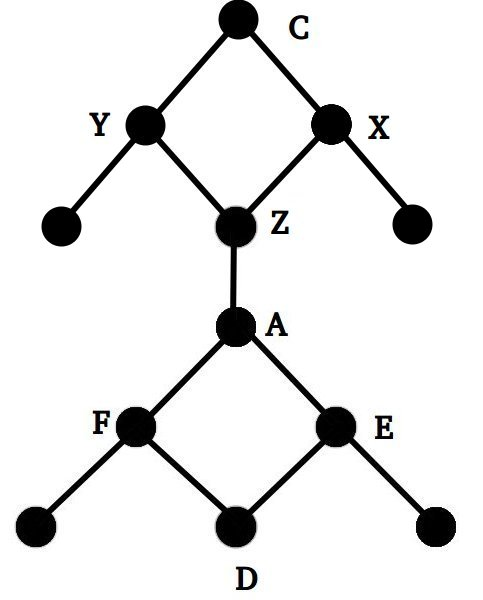
\includegraphics[scale=0.5]{example1.jpg}}
\caption{Four different paths between C and D, that share one edge.}
\label{ex1}
\end{figure}

As we mentioned earlier, sometimes we prefer to remove GCIs that involve most specific concepts during contraction. To contract such GCIs, we can just remove, from each $C-D$ path, the edges emanating from $C$. In Figure \ref{ex1}, it would mean removing two edges: (C, X) and (C, Y). But removing such edges does not guarantee the minimum change. So we might end up having to choose which strategy is more preferred: minimal change or change with most specific concepts. The minimal hitting set approach that was mentioned earlier might not always satisfy specificity. So the user might have to choose which one to apply first, and which one to use as a tie breaker.

Removing the edges that involve nodes representing most specific concepts is straightforward; remove the edges that emanate from the source node (C in our example). But it is not clear if one chooses to remove least number of edges, instead, how this can be done. For this, we introduce, in the coming section, an approach that uses the Minimum Cut algorithm to determine the minimum number edges that need to be removed and identify them.

\subsection{Reduction to network flow problem}
As explained in \cite{alg}, the network flow problem is the problem of solving a flow in a network -represented as a graph- by finding the minimum cut of the network (or the maximum flow). The input to the Ford-Fulkerson algorithm, that solves this problem, would be:
\begin{itemize}
\item A graph $G = (V, E)$.
\item A source $s \in V$.
\item A sink $t \in V$.
\item Capacity function $C:E \rightarrow \mathbb{N}$ representing the maximum capacity of each edge.
\end{itemize}

To contract $C \sqsubseteq D$ given the $TBox$ graph $G$, we choose $C$ to be the source, $D$ to be the sink, and we assume that the capacities of all edges are the same, equal to 1. The capacity is not important here, as it is normally used to determine the bottleneck edges of the network to optimize the flow, while in our case, they are only needed to determine which edges are being used; so, an edge is used in the flow if the flow passing through it is 1, and it can never be greater than 1. The algorithm will find the maximum flow from $C$ to $D$, which is equal to the capacity of the minimum cut (the sum of capacities of the cut edges); we can then extract the edges that form that minimum cut and remove them.

The approach minimum cut of the graph is equivalent to the approach of the minimal hitting set of the kernels. The minimal hitting set is the set containing the minimum number of elements that hit all sets, while the minimum cut of the graph is the minimum number of edges (since they all have the same capacity) that cover all paths from $C$ to $D$ (where edges represent GCIs of the TBox and paths represent kernels). So using the minimum cut approach should guarantee the minimum change for kernel contraction, as the minimal hitting set approach does.

Assuming we have a function ``Ford-Fulkerson(graph, s, t)" that computes the maximum flow in the network ``graph" from source node ``s" to a sink  ``t" with edge-capacities ``1", and returns the set of edges of the minimum cut, we can modify the contraction algorithm to adopt the minimum cut approach as in Algorithm \ref{GraphContract-modified}.

\begin{algorithm}
\caption{Another version of contraction algorithm}
\label{GraphContract-modified}
\begin{algorithmic}[1]
\Function {graphContractUsingMinCut}{T, A}
\State complete(T)
\State graph = transform(T)
\State $A = C \sqsubseteq D$
\State min-cut = Ford-Fulkerson(graph, C, D)
\State remove min-cut edges from graph
\State T = de-transform(graph)
\EndFunction
\end{algorithmic}
\end{algorithm}

For special cases such as contracting $C \sqsubseteq D1 \sqcap D2$, it is sufficient to contract $C \sqsubseteq D1$ first, and then contract $C \sqsubseteq D2$. But since the graph is already normalized (using complete() function), rules of the form $C \sqsubseteq D1 \sqcap D2$ are already broken down into two: $C \sqsubseteq D1$, and $C \sqsubseteq D2$. Therefore, the conjunction $\sqcap$ would only appear on the left hand side of a GCI in a normalized TBox (e.g. $A1 \sqcap A2 \sqsubseteq B$). In that case, for contracting $A1 \sqcap A2 \sqsubseteq B$, there will be a node $A1 \sqcap A2$, which we will use as a source node; the sink would be the node representing $B$. 

As in \cite{alg}, the minimum cut algorithm runs in polynomial time. So using it in the contraction algorithm will not have a significant effect on the complexity of the main algorithm (will not elevate the complexity from being polynomial to being exponential). 

In some applications, the decision about which strategy to follow for choosing the edges to remove might vary depending on the situation. So the user can be asked in such case about which strategy to follow -- specificity or minimality. 

The last step of the algorithm is to transform the graph back to $\mathcal{EL}$. This can be done as follows: starting with an empty $TBox$ $T'$, for every edge $(X, Y)$, add $X \sqsubseteq Y$ to $T'$. The resulting $TBox$ would be the result of contracting $T$ by $A$. This is discussed in Algorithm \ref{DeTransform}.

\begin{algorithm}
\caption{Transforming a graph back to a TBox}
\label{DeTransform}
\begin{algorithmic}[1]
\Function {de-transform}{graph}
\State result = $\{\}$
\State graph = (V, E)
\For{every $(X, Y) \in E$}
\State $result = result \cup \{X \sqsubseteq Y\}$
\EndFor
\State \Return result
\EndFunction
\end{algorithmic}
\end{algorithm}

Since the running time of every step of the contraction algorithm starting from ``transform(T)" until the last step is polynomial in the size of the TBox, the complexity of the algorithm will depend on the complexity of the first step (the complete() function). If building the subsumption hierarchy by generating all subsumptions of an $\mathcal{EL}$ $TBox$ can be done in polynomial time, then the contraction algorithm will in turn take polynomial time. But if generating all subsumptions takes exponential time, then the algorithm will take exponential running time as well.